\documentclass{article}
\usepackage{graphicx}
\usepackage[a4paper, left=0.8cm, right=0.8cm, top=0.80cm, bottom=0.8cm]{geometry}
\usepackage[utf8]{inputenc}
\usepackage[english,russian]{babel}
\usepackage{multicol}
\usepackage{tikz}
\usepackage{setspace}
\usepackage{array}

\newcolumntype{C}{>{\centering\arraybackslash}p{1cm}}
\usepackage{fancyhdr}

\pagestyle{fancy}
\fancyhf{}
\rhead{\thepage}

\begin{document}
	\definecolor{color1bg}{HTML}{fff2d0}
	\pagecolor{color1bg}

	\begin{multicols}{2}
		\setlength{\columnsep}{40em}
		\hspace{-15px}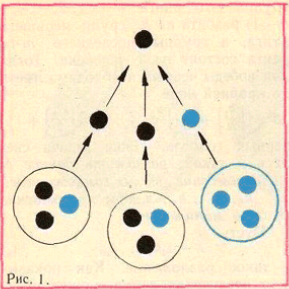
\includegraphics[width=0.45\textwidth]{Картинки/Рисунок 1.png}
		\vspace{0.5cm}
		
		\par
		\fontsize{14pt}{16pt}\selectfont
		{\small\setstretch{1.5}\textbf{M1.} В стране Анчурии, где правит 
			президент Мирафлорес, приблизилось время новых президентских выборов. В стране ровно 20 миллионов избирателей, из которых только один процент (регулярная армия Анчурин) поддерживает Мирафлореса. Мирафлорес, естественно, хочет быть избранным, но, с другой стороны, он хочет, чтобы выборы казались демократическими. «Демократическим голосованием» Мирафлорес называет вот что: все избиратели разбиваются на несколько равных групп, затем каждая из этих групп вновь разбивается на некоторое количество равных групп, затем эти последние группы снова разбиваются на равные группы и т. д.; в самых мелких группах выбирают представителя группы-выборщика, затем выборщики выбирают представителей для голосования в еще большей группе и т. д.; наконеп, представители самых больших групп выбирают президента. Мирафлорес делит избирателей на группы, как он хочет, и инструктирует своих сторонников, как им голосовать. Сможет ли он так организовать «демократические выборы», чтобы его избрали президентом? (При равенстве голосов побеждает оппозиция.)}
		
		\par
		О т в е т. \emph{Да, сможет.}
		\par 
		Прежде всего, разберемся, как может на «многоступенчатых» выборах
		%\columnbreak
		победить кандидат, за которого голосует меньшинство. (Кстати, по такой системе голосуют во многих капиталистических странах.) Самый простой пример такой ситуации изображен на рисунке 1: здесь девять избирателей - четыре «черных» и пять «голубых» - разбиты на три группы по три избирателя так, что в двух группах побеждают черные, и поэтому в результате таких «двухступенчатых выборов» будет избран кандидат черных, хотя число его сторонников сос-
		тавляет только \Large{$\frac{4}{5}$} от общего числа 5
		избирателей. (Нетрудно сообразить, что при двухступенчатых выборах с большим числом избирателей процент голосов, достаточный для победы, может быть еще меньше, но всетаки заведомо больше 25\%.) Ясно, что при трехступенчатой системе выборов этот процент можно сделать еще ниже. Например, если заменить на рисунке 1 каждого избирателя группой из ста человек, причем так, что в голубой группе все сто избирателей голубые, а в черной - 51 черный и 49 голубых, то мы получим пример ситуации, где черные состав- 51 17 ляют только \Large{$\frac{4}{9} \cdot \frac{51}{100}$ = $\frac{17}{75}$}  от общего числа избирателей и тем не менее побеж-
		дают.
		\par
		После этих предварительных соображений приведем решение задачи. 
		\par
		Разобьем всех избирателей на 5 групп по 4 миллиона в каждой так, что две группы целиком состоят из противников Мирафлореса (назовем эти группы «голубыми», а три остальные - «черными»). Каждую из
	\end{multicols}
	
	
	
	\hspace{-15px}\begin{tabular}{p{6cm} C C C C C C C C C}
		\hline
		&&&&&&&&&\\
		Ранг группы r & 1 & 2 & 3 & 4 & 5 & 6 & 7 & 8 & 9\\
		Общее число групп ранга & 5 & $5^2$ & $5^3$ & $5^4$ & $5^5$ & $5^6$ & $5^7$ & $2^4 \cdot 5^7$ & $2^8 \cdot 5^7$\\
		Сколько из них черных & 3 & $3^2$ & $3^3$ & $3^4$ & $3^5$ & $3^6$ & $3^7$ & $3^9$ & $3^11$\\
		Сколько человек в одной группе ранга r & $4 \cdot 10^6$ & $8 \cdot 10^5$ & $16 \cdot 10^4$ & $32 \cdot 10^3$ & $64 \cdot 10^2$ & 1280 &256 & 16 & 1\\
		На сколько групп ранга (r + 1) разбивается каждая группа ранга & 5 & 5 & 5 & 5 & 5 & 5 & 16 & 16 & - \\
		Сколько черных подгрупп ранга (r + 1) у черной группы ранга г & 3 & 3 & 3 & 3 & 3 & 3 & 9 & 9 & - \\
		&&&&&&&&&\\
		\hline
		
	\end{tabular}
	\begin{flushright}
		\textbf{49}
	\end{flushright}
	
	\newpage
	\begin{multicols}{2}
		\hspace{-15px}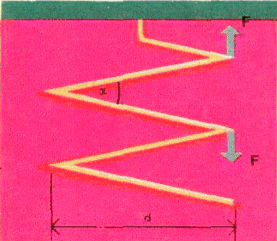
\includegraphics[width=0.45\textwidth]{Картинки/Рисунок 11.png}
		\vspace{-1cm}
		\par
		\hspace{-17px} Рис. 11.
		\par
		\vspace{-1cm}
		\hspace{-21px}
		жесткость всей пружины. Поэтому \Large{$c_{2} = \frac{m_{1} + m_{2}}{m_{2}}$} Отсюда следует, что период колебаний шариков
		\Large{$\emph{T} = 2\pi \sqrt{\frac{m_{1}m_{2}}{(m_{1} + m_{2}) \cdot c}}$}
		Интересно проверить ответ, взяв какой-нибудь предельный случай. Так поступил ученик 10 класса школы № 20 из г. Вологды Е. \emph{Тихонов.} Предположим, что масса т, очень велика: \Large{$m_{2} \gg m_{1}$}. Тогда шарик с массой т1 должен колебаться так, как если бы второй шар был неподвижно закреплен, и
		\Large{$\emph{T} =  \sqrt{\frac{m_{1}}{c}}$}
		Проверим нашу формулу\\
		\Large{$\emph{T} = 2\pi \sqrt{\frac{m_{1}}{c(1 + \frac{m_{1}}{m_{2}})}} \approx 2\pi \sqrt{\frac{m_{1}}{c}}$}
		\vspace{-1cm}
		\par
		{\small\textbf{ФЗ.} Из двух одинаковых кусков стальной проволоки свили две пружины. Диаметр витков одной из них равен d, другой 2d. Первая пружина под действием груза растянулась на одну десятую своей длины. На какую часть своей длины растянется под действием того же груза вторая пружина?}
		\vspace{-1cm}
		\par
		Удлинение пружины равно\\ $\triangle l = n \cdot 2d \cdot \sin{\frac{\alpha}{2}}$, где \emph{n} - число вит-
		ков пружины, а а - угол, на который разворачиваются соседние витки пружины (рис. 11). Так как удлинение пружины мало, то этот угол мал и\\
		\Large{$\sin{\frac{\alpha}{2}} \approx \frac{\alpha}{2}$} Поэтому \Large{$\triangle l = nd\alpha$}.
		\vspace{-1cm}
		\par
		Угол $\alpha$ пропорционален моментам
		\columnbreak
		сил \emph{F}, которые растягивают виток: $\alpha = F \cdot d$. Сила \emph{F} равна весу груза, подвешенного к пружине, и одинакова в обоих случаях, поэтому $\triangle l \sim dn^2$.
		Диаметр витков второй пружины вдвое больше, а число витков у нее вдвое меньше, следовательно, абсолютное удлинение второй пружины вдвое больше, чем у первой. Таким образом, вторая пружина растянет-
		ся на $\frac{2}{5}$ - своей длины.
		Многие, приславшие решение этой задачи, правильно нашли, что удлинение второй пружины в два раза больше, чем первой, но забыли, что вторая пружина вдвое короче, чем первая, поэтому относительное удлинение второй пружины равно не
		как получалось у них, $a \cdot \frac{2}{5}$
		\par
		{\small\textbf{Ф4.} В баллоне содержится очищенный газ, но неизвестно какой. Чтобы поднять температуру 1 кг этого газа на один градус при постоянном давлении требуется 958,4 \emph{дж}, а при постоянном объеме - 704,6 \emph{дж}. Что это за газ?}
		\par
		При нагревании газа при постоянном объеме затрачиваемая энергия идет только на изменение внутренней энергии газа, а при нагревании при постоянном давлении - еще и на совершение работы. Запишем закон сохранение энергии для обоих случаев:\\
		\[mc_{V}\triangle t = \triangle W, \hspace{12px}(1)\] 
		\[mc_{p}\triangle t = \triangle W + A.\hspace{12px}(2)\]\\
		Здесь $c_{p}$ - теплоемкость газа при постоянном давлении (т. е. количество тепла, которое необходимо для нагревания 1 \emph{кг} газа при постоянном давлении), $c_{V}$ - теплоемкость газа при постоянном объеме, $\triangle t$ - изменение температуры, $\triangle W$ - изменение внутренней энергии газа, \emph{m} - масса газа, $A = p\triangle V$ - совершенная при расширении газа работа ($\triangle V$ - изменение объема, \emph{p} - давление).
		Так как при повышении температуры газа на одинаковое число градусов изменение его внутренней энергии одинаково как при нагревании при постоянном объеме, так и при \hfill {\small\textbf{52}}
	\end{multicols}
	
\end{document}


